\documentclass[11pt,a4paper]{article}

\usepackage[utf8]{inputenc}
\usepackage[T1]{fontenc}
\usepackage{lmodern}
\usepackage{CJKutf8}
\usepackage{microtype}
\usepackage{amsmath, amssymb}
\usepackage{mathtools}
\usepackage{booktabs}
\usepackage{array}
\usepackage{tabularx}
\usepackage{multirow}
\usepackage{xcolor}
\usepackage{tikz}
\usepackage{pgfplots}
\pgfplotsset{compat=1.18}
\usetikzlibrary{arrows.meta, positioning, shapes.geometric, fit, backgrounds, calc, patterns}
\usepackage{float}
\usepackage{hyperref}
\usepackage[numbers,sort&compress]{natbib}
\usepackage{geometry}
\usepackage{listings}
\usepackage{enumitem}
\usepackage{titlesec}
\usepackage{abstract}

\geometry{
  top=2.5cm, bottom=2.5cm,
  left=2.5cm, right=2.5cm
}

\hypersetup{
  colorlinks=true,
  linkcolor=blue!60!black,
  citecolor=green!50!black,
  urlcolor=blue!70!black
}

\lstset{
  basicstyle=\small\ttfamily,
  backgroundcolor=\color{gray!10},
  frame=single,
  framesep=4pt,
  breaklines=true,
  columns=fullflexible,
  keepspaces=true,
  xleftmargin=0.5em,
  xrightmargin=0.5em
}

\newcommand{\R}{\mathbb{R}}
\newcommand{\St}{S_t}
\newcommand{\Stp}{S_{t+1}}
\newcommand{\wstd}{w_{\mathrm{std}}}

\title{
  \textbf{Persistent Latent Modulation in Frozen LLMs:}\\[0.3em]
  \large From Additive Bottleneck to Multiplicative Symmetry Breaking\\[0.2em]
  \normalsize\textit{Structural Differentiation Without Functional Coupling}
}

\author{
  Xiao Ouyang \textup{(\begin{CJK}{UTF8}{gbsn}欧阳潇\end{CJK})}
}

\date{\today}

\begin{document}

\maketitle
\thispagestyle{empty}

\begin{abstract}
We study whether a persistent learnable latent state can control the computation of a
frozen pretrained LLM (Qwen3-4B) through residual-stream modulation, and we
systematically compare three injection mechanisms. \textbf{(1)~Additive gated
cross-attention} ($h_s + \mathrm{gate}\cdot e_o$) is causally negligible: the maximum
ablation effect ($\Delta\mathrm{PPL} = 2.01$) is below the measurement noise floor
($\mathrm{std}=\pm 19$), because the residual stream robustly absorbs additive
perturbations. \textbf{(2)~AdaLN-style FiLM} appeared, in preliminary testing, to be
strongly causal ($\Delta = 11.44$ upon removal). We show this measurement was an
artifact of two compounding errors---a composite training loss and a checkpoint
persistence bug that silently evaluated against zero-valued modulation weights. After
correction, the pure language-modeling causal effect is unverifiable and, on the
multiplicative variant, essentially zero. \textbf{(3)~Multiplicative FiLM}
($h_s \times (1+\alpha\tanh(W_\ell S_t))$) induces a spontaneous symmetry-breaking
transition: inter-layer modulation variance ($\wstd$) grows monotonically from $0.06$
to $0.40$ ($6.6\times$) over 2{,}650 steps. Yet a controlled ablation with
\emph{verified non-zero} weights reveals a sharp \textbf{dissociation between structure
and function}: removing FiLM changes pure LM loss by only $\Delta = 0.044$, and
freezing the latent state $\St$ by $\Delta = 0.0002$---the dominant task improvement
($3.53 \to 2.70$, $-24\%$) comes from concurrently trained PEFT adapters, not from the
modulation. We conclude that weight-space symmetry breaking and output-space causal
control are \emph{separable} phenomena: layers can differentiate structurally while
remaining functionally near-identical, and the persistent latent state---the core
premise of this architecture---is computationally inert under bounded
($\alpha = 0.1$) modulation. We close with a methodological warning: weight-space
metrics are misleading proxies for functional influence absent causal ablation with
verified weights.
\end{abstract}

\newpage
\setcounter{page}{1}

%------------------------------------------------------------------
\section{Introduction}
%------------------------------------------------------------------

Large language models process all inputs through a uniform residual
stream\footnote{Residual stream: the sequence of hidden-state vectors passed
additively between transformer layers, serving as the primary information pathway
through the network.} in which each token effectively re-initializes the computational
state. This design achieves remarkable local reasoning but provides no mechanism for
\textbf{persistent internal state}---latent variables that evolve across tokens and
modulate computation accordingly.

This paper asks a concrete question: \emph{can a learnable latent state $\St$, injected
into a frozen LLM, exert genuine causal influence on the model's output?} We study
this through a frozen Qwen3-4B backbone augmented with a GRU-evolved latent state
$\St \in \R^{256}$, and we compare three families of injection mechanism that span the
additive--multiplicative design space.

\textbf{The arc of this paper is also a cautionary tale.} Our initial experiments
suggested that one mechanism (AdaLN FiLM) achieved strong causal control
($\Delta = 11.44$). On investigation, this number turned out to be the product of two
methodological errors: (i)~the causal ``loss'' was a \emph{composite} objective that
mixed the language-modeling term with auxiliary regularizers, and (ii)~a
\textbf{checkpoint persistence bug} caused all early ablations to silently load
zero-valued modulation weights. Correcting both reverses the headline conclusion. We
present the corrected analysis here and treat the original $11.44$ strictly as an
invalidated artifact.

\textbf{Key contributions.}

\begin{enumerate}[leftmargin=*, label=\textbf{\arabic*.}]

  \item \textbf{Additive injection is structurally weak.}
    Gated cross-attention\footnote{Cross-attention: queries from one representation
    attend to keys and values from another, enabling information flow between
    heterogeneous feature spaces.} ($h_s + \mathrm{gate}\cdot e_o$) is causally
    negligible ($\Delta\mathrm{PPL}\footnote{Perplexity (PPL): a standard language-model
    quality metric, $2^{H}$ where $H$ is the cross-entropy. Lower is better;
    differences ($\Delta$PPL) measure the causal impact of an intervention.} = 2.01$
    vs.\ noise $\mathrm{std} = \pm 19$). Transformer residual streams absorb additive
    perturbations.

  \item \textbf{A measurement artifact, corrected.}
    The apparent strong control of AdaLN FiLM ($\Delta = 11.44$) is shown to arise from
    a composite loss and a checkpoint persistence bug. With verified non-zero weights
    and pure LM loss, multiplicative FiLM's causal effect is $\Delta = 0.044$.

  \item \textbf{Structural symmetry breaking.}
    Multiplicative FiLM induces $6.6\times$ growth in inter-layer modulation variance
    ($\wstd: 0.06 \to 0.40$) with gradient decoupling (cosine similarity
    $0.99 \to 0.34$).

  \item \textbf{Dissociation of structure and function.}
    Despite this structural differentiation, the layers' actual effect on output is
    near-identical: causal $\Delta = 0.044$. Weight-space and function-space
    differentiation are separable phenomena.

  \item \textbf{Negative result on the persistent latent state.}
    Freezing $\St$ changes output by $\Delta = 0.0002$. The persistent state is
    computationally inert under bounded modulation.

  \item \textbf{Methodological contribution.}
    We document a silent failure mode of PEFT\footnote{Parameter-Efficient Fine-Tuning
    (PEFT): training a small subset of parameters while keeping the base model frozen.}
    research---\texttt{save\_pretrained()} does not persist custom injection layers---and
    the corrected evaluation protocol.

\end{enumerate}

%------------------------------------------------------------------
\section{Method}
%------------------------------------------------------------------

\subsection{State Pipeline}

The latent state $\St \in \R^{256}$ evolves via a GRU cell\footnote{Gated Recurrent
Unit (GRU)~\cite{cho2014learning}: a recurrent cell using update and reset gates for
smooth state transitions with fewer parameters than LSTM.} conditioned on the
transformer's final hidden state at the last non-padded token position. The initial
state $S_0$ is a learned parameter with Gaussian noise ($\sigma = 0.01$) for symmetry
breaking.

\[
  S_0 \;\to\; \text{each turn:}\quad
  h_s \times (1+\alpha\tanh(W_\ell \St)) \;\to\; \mathrm{forward} \;\to\; h_t
  \;\to\; \Stp = \mathrm{GRU}(\St,\, h_t)
\]

\begin{figure}[H]
\centering
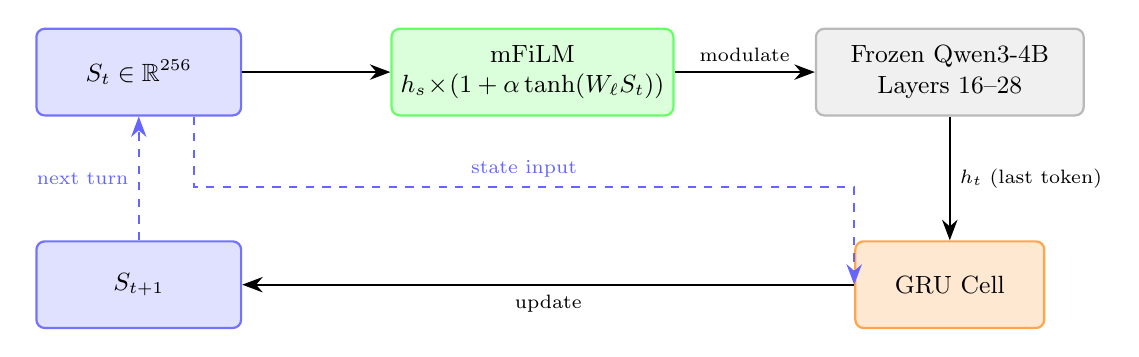
\begin{tikzpicture}[
  font=\small,
  box/.style={rectangle, draw, rounded corners=3pt, minimum height=11mm, align=center, thick},
  state/.style={box, fill=blue!12, draw=blue!55, minimum width=26mm},
  film/.style={box, fill=green!14, draw=green!60, minimum width=34mm},
  tf/.style={box, fill=gray!12, draw=gray!55, minimum width=34mm},
  gru/.style={box, fill=orange!18, draw=orange!70, minimum width=24mm},
  flow/.style={-{Stealth[length=2.6mm]}, thick},
  fb/.style={-{Stealth[length=2.6mm]}, thick, dashed, blue!60}
]
\node[state] (st)   at (0,0)     {$S_t \in \mathbb{R}^{256}$};
\node[film]  (film) at (5.0,0)   {mFiLM\\$h_s\!\times\!(1+\alpha\tanh(W_\ell S_t))$};
\node[tf]    (tf)   at (10.3,0)   {Frozen Qwen3-4B\\Layers 16--28};
\node[gru]   (gru)  at (10.3,-2.7) {GRU Cell};
\node[state] (stp)  at (0,-2.7)   {$S_{t+1}$};

\draw[flow] (st)   -- (film);
\draw[flow] (film) -- node[above, font=\scriptsize] {modulate} (tf);
\draw[flow] (tf)   -- node[right, font=\scriptsize] {$h_t$ (last token)} (gru);
\draw[flow] (gru)  -- node[below, font=\scriptsize] {update} (stp);
% current state also feeds the GRU as recurrent input
\draw[fb] ($(st.south)+(0.7,0)$) -- ++(0,-0.9)
          -| node[pos=0.25, above, font=\scriptsize] {state input} (gru.west);
% next-turn state becomes the current state (persistence loop)
\draw[fb] (stp) -- node[left, font=\scriptsize] {next turn} (st);
\end{tikzpicture}
\caption{PLAA state pipeline with multiplicative FiLM. The latent state $S_t$ gates the
feature amplitude of frozen transformer layers $16$--$28$; the output hidden state
$h_t$ updates the state via a GRU cell, producing $S_{t+1}$ for the next turn. The
dashed loop is the persistence channel that makes $S_t$ the only cross-turn carrier.}
\label{fig:architecture}
\end{figure}

\subsection{Three Injection Mechanisms}

We study three mechanisms on the same backbone, data, and layer set ($16$--$28$,
i.e.\ $13$ injected layers).

\subsubsection*{(1) Additive Gated Cross-Attention}

\begin{lstlisting}
Each injected layer:
  Self-Attn -> EmotionCrossAttn(Q=hidden, K,V=proj(S_t))
            -> GatedResidual(h + gate * eo)   # additive
            -> MLP
\end{lstlisting}
with $\mathrm{gate}\in\R$ ($\tanh$, init $0.1$) and $e_{\mathrm{mem}}=\mathrm{proj}(\St)\in\R^{16\times2560}$.

\subsubsection*{(2) AdaLN FiLM}

\begin{lstlisting}
Each injected layer:
  Self-Attn -> AdaLN( LN(hs) * (1 + scale(S)) + shift(S) )
            -> MLP
\end{lstlisting}
with $\mathrm{scale}=\alpha\tanh(W_{\mathrm{scale}}\St)$, $\mathrm{shift}=\alpha\tanh(W_{\mathrm{shift}}\St)$, $\alpha=0.1$.

\subsubsection*{(3) Multiplicative FiLM (primary architecture)}

\begin{lstlisting}
Each injected layer:
  Self-Attn -> hs = hs * (1 + alpha * tanh(W_l * S_t))   # multiplicative gain
            -> MLP
\end{lstlisting}

Key design choices: \textbf{per-layer projections} ($W_\ell\in\R^{2560\times256}$,
independent per layer); \textbf{zero initialization} of $W_\ell$ so modulation starts
as identity ($h_s\times1$) and specialization must be learned; \textbf{pure
multiplicative gain} on the unnormalized hidden state; and a fixed bound $\alpha=0.1$
throughout training.

\subsection{Training Data}

Training uses 3{,}197 dialogue micro-trajectories ($3$--$5$ turns each), stratified
$60{:}30{:}10$:

\begin{table}[h]
\centering
\begin{tabular}{clll}
\toprule
\textbf{Ratio} & \textbf{Source} & \textbf{Purpose} \\
\midrule
60\% & PersonaChat (neutral)      & Latent continuity  \\
30\% & ESConv (emotional support) & Gradual trajectory \\
10\% & Synthetic roleplay         & Dynamic range      \\
\bottomrule
\end{tabular}
\caption{Training data composition.}
\end{table}

\subsection{Optimization}

\begin{table}[h]
\centering
\begin{tabular}{ll}
\toprule
\textbf{Hyperparameter} & \textbf{Value} \\
\midrule
Base model         & Qwen3-4B (frozen) \\
Quantization       & NF4 (4-bit), SDPA attention \\
Trainable params   & 17.5M (FiLM projections + GRU) \\
Optimizer          & AdamW,\quad lr $=1\times10^{-4}$ \\
Batch size         & 2 \\
Total steps        & 2{,}650 \\
$\alpha$ (modulation bound) & 0.1 \\
GPU                & NVIDIA RTX PRO 6000 Blackwell (96\,GB) \\
\bottomrule
\end{tabular}
\caption{Training configuration. The composite training loss is
$\mathcal{L} = \mathcal{W}_{\mathrm{LM}}\mathcal{L}_{\mathrm{LM}}
+ \mathcal{W}_{\mathrm{COH}}\|\Delta S\|
+ \mathcal{W}_{\mathrm{DIV}}\mathcal{L}_{\mathrm{repulsion}}
+ \mathcal{W}_{\mathrm{NORM}}\|S\|
+ \mathcal{W}_{\mathrm{DIV\_LAYER}}\mathrm{Var}(\|W_\ell\|)$;
crucially, all \emph{causal} evaluations in this paper use the pure LM term
$\mathcal{L}_{\mathrm{LM}}$ only (see Section~\ref{sec:bug}).}
\end{table}

\subsection{Metrics}

\begin{itemize}
  \item $\wstd$: standard deviation of $\|W_\ell\|$ across layers $16$--$28$.
    Measures \emph{structural} differentiation.
  \item \textbf{cos}: mean pairwise cosine similarity\footnote{Cosine similarity:
    $\cos\theta = \mathbf{a}\cdot\mathbf{b}/(\|\mathbf{a}\|\|\mathbf{b}\|)$; $1$ is
    parallel, $0$ orthogonal.} of per-layer gradient updates. Measures inter-layer
    coupling.
  \item \textbf{Causal $\Delta$}: change in \emph{pure} LM cross-entropy when a
    component is ablated. Measures \emph{functional} influence.
\end{itemize}

%------------------------------------------------------------------
\section{The Additive Bottleneck}
%------------------------------------------------------------------

We first establish that additive gated cross-attention is causally insufficient.

\subsection{Gate Gradient Diagnostic and Multi-Stage Attenuation}

A gate-gradient probe at step $1350$ confirms a live gradient path
(\texttt{avg gate.grad} $= 0.056$, non-zero). Yet the effective signal is attenuated
in three compounding stages:

\begin{enumerate}
  \item $\|\St\| \approx 0.15$ (from the norm penalty) $\Rightarrow$ small projection;
  \item $\tanh(\mathrm{gate}=0.1) \approx 0.1$ further attenuates;
  \item $\times 13$ residual-stack integrations $\Rightarrow$ effective influence
    $\approx 0.0003\cdot\|h_{\mathrm{hidden}}\|$.
\end{enumerate}

\subsection{Gate Ablation}

\begin{table}[h]
\centering
\begin{tabular}{lcc}
\toprule
\textbf{Condition} & \textbf{PPL} & \textbf{$\Delta$PPL} \\
\midrule
gate $= 0$      & 27.03 & ---  \\
gate $= 1.0$    & 26.26 & 0.77 \\
gate $= 2.0$    & 25.02 & 2.01 \\
gate $=$ random & 25.94 & 1.09 \\
\bottomrule
\end{tabular}
\caption{Gate ablation. Maximum $\Delta\mathrm{PPL} = 2.01$, against measurement noise
$\mathrm{std} = \pm 19$. Causal influence is below the noise floor.}
\label{tab:gate}
\end{table}

\textbf{Conclusion.} Additive injection is causally insufficient; the residual stream
absorbs additive perturbations. This is the motivating failure that prompts the move to
\emph{multiplicative} conditioning.

%------------------------------------------------------------------
\section{AdaLN FiLM and the Checkpoint Persistence Bug}
\label{sec:bug}
%------------------------------------------------------------------

\subsection{An Apparent (but Invalid) Strong Result}

AdaLN-style modulation~\cite{perez2018film, peebles2023scalable} initially appeared to
achieve strong causal control: removing it raised the measured loss from $14.68$ to
$3.14$, an apparent $\Delta = 11.44$. \textbf{This measurement is invalid.} Two
compounding errors inflated it, and we report it only to document the correction.

\subsection{The Two Errors}

\textbf{Error 1: composite loss.} The $14.68$ ``loss'' was the full composite training
objective (LM $+$ coherence $+$ repulsion $+$ norm terms), not pure language-modeling
cross-entropy. Removing FiLM also perturbs the auxiliary terms, producing a large but
meaningless delta.

\textbf{Error 2: checkpoint persistence bug.} PEFT's \texttt{save\_pretrained()}
persists only LoRA adapter weights, \emph{not} custom injection layers. All early
ablations therefore loaded checkpoints with zero-valued \texttt{scale\_proj}
weights---the FiLM modulation was silently disabled during evaluation. We corrected
this by serializing the injection weights separately:

\begin{lstlisting}
torch.save({
    "plaa_core": plaa_core.state_dict(),
    "scale_proj": {i: layer_blocks[i].scale_proj.state_dict()
                   for i in range(16, 29)},
}, f"{ckpt_dir}/plaa_core.pt")
\end{lstlisting}

Verified checkpoint (step $850$): scale-norm sum $= 74.41$, $\wstd = 0.307$; weights
confirmed non-zero and structurally differentiated.

\subsection{Corrected Causal Ablation (Pure LM Loss, Verified Weights)}

\begin{table}[h]
\centering
\begin{tabular}{lcc}
\toprule
\textbf{Condition} & \textbf{Pure LM Loss} & $\boldsymbol{\Delta}$ \textbf{vs.\ trained} \\
\midrule
Vanilla Qwen3-4B (no adapters, no FiLM)      & 3.534 & --- \\
Trained system (LoRA + mFiLM, normal $S$)    & 2.700 & $-0.834$ vs.\ vanilla \\
FiLM removed (scale forced to 0)             & 2.744 & $+0.044$ \\
State frozen ($S = S_0$, FiLM active)        & 2.700 & $+0.0002$ \\
\bottomrule
\end{tabular}
\caption{Causal ablation with verified non-zero FiLM weights, pure LM cross-entropy
(no auxiliary terms). The corrected story is the opposite of the artifact: removing
FiLM costs only $+0.044$; freezing the latent state costs $+0.0002$.}
\label{tab:causal}
\end{table}

This corrected ablation is visualized in Figure~\ref{fig:ablation}.

\begin{figure}[H]
\centering
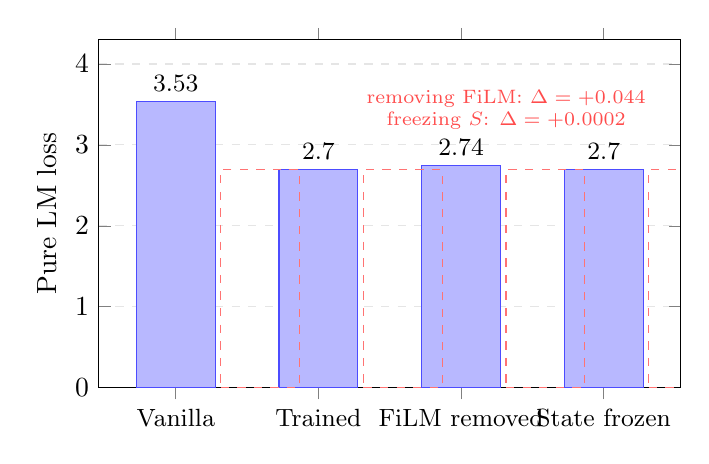
\begin{tikzpicture}
\begin{axis}[
  ybar,
  width=0.74\linewidth, height=6cm,
  ylabel={Pure LM loss},
  symbolic x coords={Vanilla, Trained, {FiLM removed}, {State frozen}},
  xtick=data,
  x tick label style={font=\small, align=center},
  ymin=0, ymax=4.3,
  ytick={0,1,2,3,4},
  bar width=1.0cm,
  enlarge x limits=0.18,
  ymajorgrids=true, grid style={gray!20, dashed},
]
\addplot[fill=blue!28, draw=blue!70,
         nodes near coords, nodes near coords style={font=\small\bfseries}]
  coordinates {(Vanilla,3.534) (Trained,2.700) ({FiLM removed},2.744) ({State frozen},2.700)};
% reference line at the trained level: the three right bars sit on it
\addplot[dashed, red!55, no marks, forget plot] coordinates {
  (Vanilla,2.700) (Trained,2.700) ({FiLM removed},2.700) ({State frozen},2.700)};
\node[font=\scriptsize, red!70, anchor=center, align=center]
  at (rel axis cs:0.70,0.80)
  {removing FiLM: $\Delta=+0.044$\\ freezing $S$: $\Delta=+0.0002$};
\end{axis}
\end{tikzpicture}
\caption{Corrected causal ablation. The $24\%$ improvement over vanilla
($3.53\!\to\!2.70$) comes from the LoRA adapters; removing FiLM or freezing the latent
state leaves the loss essentially unchanged (red reference line at the trained level).
The previously reported $\Delta=11.44$ for AdaLN FiLM was a composite-loss/checkpoint-bug
artifact and is \emph{not} shown here.}
\label{fig:ablation}
\end{figure}

%------------------------------------------------------------------
\section{Multiplicative FiLM: Structural Symmetry Breaking}
%------------------------------------------------------------------

Switching to multiplicative FiLM triggers an immediate and sustained growth in
layer-wise structural differentiation---even though, as Section~\ref{sec:bug} shows,
this does not translate into functional control.

\subsection{Layer Specialization Growth}

\begin{table}[h]
\centering
\begin{tabular}{cc}
\toprule
\textbf{Step} & $\boldsymbol{\wstd}$ \\
\midrule
   50 & 0.062 \\
  350 & 0.244 \\
  800 & 0.333 \\
 1800 & 0.356 \\
 2650 & 0.404 \\
\bottomrule
\end{tabular}
\caption{Monotonic growth of inter-layer modulation variance: $6.6\times$ over
2{,}650 steps, with no saturation plateau. Contrast the additive/AdaLN plateau of
$\wstd = 0.033$.}
\label{tab:wstd}
\end{table}

Growth is monotonic across all $53$ recorded checkpoints
(Figure~\ref{fig:wstd-growth}).

\begin{figure}[H]
\centering
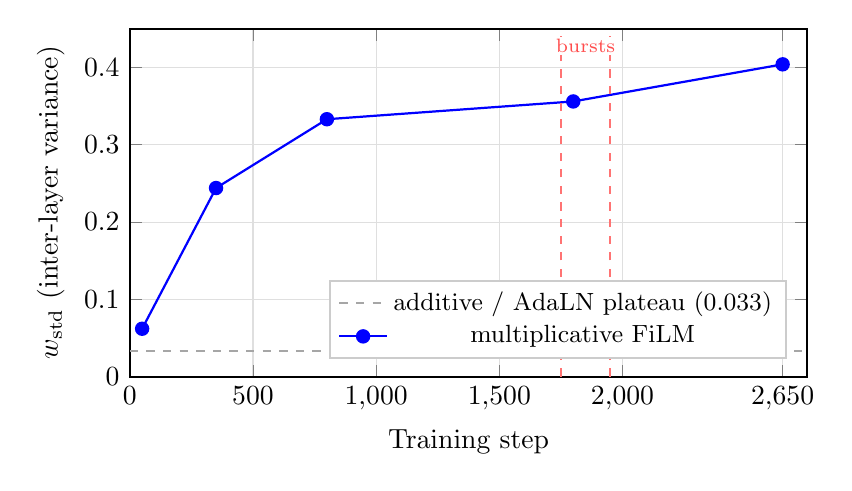
\begin{tikzpicture}
\begin{axis}[
  width=0.84\linewidth, height=6cm,
  xlabel={Training step}, ylabel={$\wstd$ (inter-layer variance)},
  xmin=0, xmax=2750, ymin=0, ymax=0.45,
  xtick={0,500,1000,1500,2000,2650},
  ytick={0,0.1,0.2,0.3,0.4},
  grid=major, grid style={gray!25},
  legend style={at={(0.97,0.05)}, anchor=south east, font=\small, draw=gray!40, fill=white},
  thick,
]
% additive / AdaLN plateau reference
\addplot[dashed, gray!70, no marks] coordinates {(0,0.033) (2750,0.033)};
\addlegendentry{additive / AdaLN plateau (0.033)}
\addplot[blue, mark=*, mark size=2.2pt, thick] coordinates {
  (50,0.062) (350,0.244) (800,0.333) (1800,0.356) (2650,0.404)};
\addlegendentry{multiplicative FiLM}
% regime-hopping bursts: w_std keeps rising during cosine spikes
\draw[red!55, dashed] (axis cs:1750,0) -- (axis cs:1750,0.45);
\draw[red!55, dashed] (axis cs:1950,0) -- (axis cs:1950,0.45);
\node[font=\scriptsize, red!70, anchor=south, fill=white, inner sep=0.8pt]
  at (axis cs:1850,0.415) {bursts};
\end{axis}
\end{tikzpicture}
\caption{Structural symmetry breaking. Inter-layer modulation variance $\wstd$ grows
monotonically ($6.6\times$), far above the additive/AdaLN plateau (gray dashed). During
the two synchronization bursts (red dashed, steps $1750$/$1950$, where gradient cosine
spikes to $0.63$/$0.70$), $\wstd$ does \emph{not} collapse---it continues rising
($0.348\!\to\!0.382$), and loss recovers to a lower attractor afterward.}
\label{fig:wstd-growth}
\end{figure}

\subsection{Phase-Plane Dynamics and Regime Hopping}

In the $\wstd$--cos phase plane the system traces a characteristic trajectory: an
early rise ($\wstd\to0.24$, cos $0.35$--$0.61$), a temporary mid plateau
($\wstd\approx0.33$, cos $0.34$--$0.63$), and a late resumption
($\wstd\to0.40$, cos $0.42$--$0.63$). Two synchronization bursts (step $1750$:
cos $=0.627$; step $1950$: cos $=0.696$) momentarily increase global coupling without
collapsing $\wstd$, after which loss recovers to a lower baseline
($10.4\to5.3$)---a metastable, self-recovering hierarchy.

\begin{figure}[H]
\centering
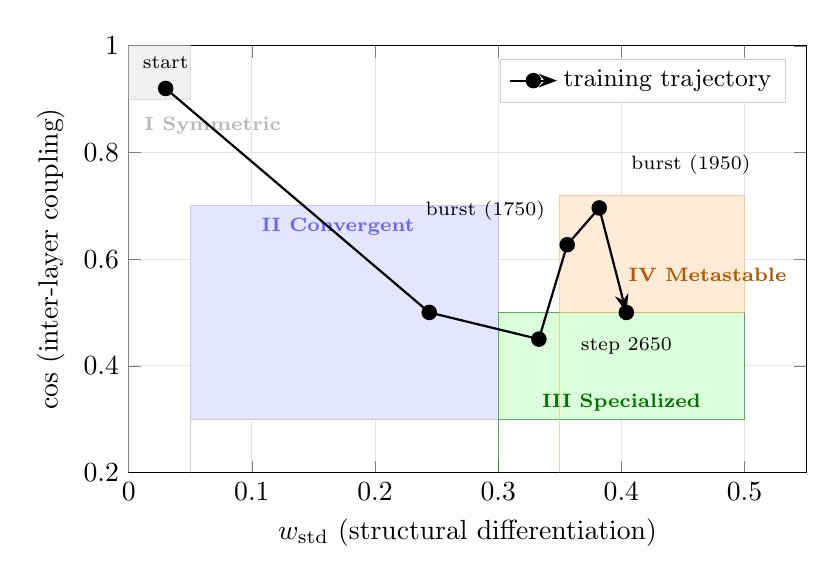
\begin{tikzpicture}
\begin{axis}[
  width=0.84\linewidth, height=7cm,
  xlabel={$\wstd$ (structural differentiation)},
  ylabel={cos (inter-layer coupling)},
  xmin=0, xmax=0.55, ymin=0.2, ymax=1.0,
  xtick={0,0.1,0.2,0.3,0.4,0.5},
  ytick={0.2,0.4,0.6,0.8,1.0},
  grid=major, grid style={gray!20},
  legend style={at={(0.97,0.97)}, anchor=north east, font=\small, draw=gray!40, fill=white},
  clip=false,
]
% phase regions
\addplot[fill=gray!12, draw=gray!45, draw opacity=0.6, forget plot]
  coordinates {(0,0.9) (0.05,0.9) (0.05,1.0) (0,1.0)} \closedcycle;
\node[font=\scriptsize\bfseries, gray!55, anchor=west] at (axis cs:0.005,0.85) {I Symmetric};
\addplot[fill=blue!10, draw=blue!35, draw opacity=0.6, forget plot]
  coordinates {(0.05,0.3) (0.3,0.3) (0.3,0.7) (0.05,0.7)} \closedcycle;
\node[font=\scriptsize\bfseries, blue!60] at (axis cs:0.17,0.66) {II Convergent};
\addplot[fill=green!14, draw=green!45!black, draw opacity=0.6, forget plot]
  coordinates {(0.3,0.3) (0.5,0.3) (0.5,0.5) (0.3,0.5)} \closedcycle;
\node[font=\scriptsize\bfseries, green!45!black] at (axis cs:0.40,0.33) {III Specialized};
\addplot[fill=orange!16, draw=orange!60, draw opacity=0.6, forget plot]
  coordinates {(0.35,0.5) (0.5,0.5) (0.5,0.72) (0.35,0.72)} \closedcycle;
\node[font=\scriptsize\bfseries, orange!70!black] at (axis cs:0.47,0.57) {IV Metastable};
% trajectory through the phase plane
\addplot[thick, black, mark=*, mark size=2.4pt, -{Stealth}]
  coordinates {(0.03,0.92) (0.244,0.50) (0.333,0.45) (0.356,0.627) (0.382,0.696) (0.404,0.50)};
\addlegendentry{training trajectory}
\node[font=\scriptsize, anchor=south] at (axis cs:0.03,0.94) {start};
\node[font=\scriptsize, anchor=south east] at (axis cs:0.346,0.655) {burst (1750)};
\node[font=\scriptsize, anchor=south west] at (axis cs:0.40,0.74) {burst (1950)};
\node[font=\scriptsize, anchor=north] at (axis cs:0.404,0.47) {step 2650};
\end{axis}
\end{tikzpicture}
\caption{$\wstd$--cos phase plane. The system departs the symmetric corner (Phase~I,
homogeneous layers) and settles into Phase~IV, a metastable coupled hierarchy, via
intermittent synchronization bursts. Phase classification here is \emph{structural}
only; the causal ablation (Figure~\ref{fig:ablation}) shows this differentiation does
not entail functional specialization.}
\label{fig:phase-plane}
\end{figure}

\subsection{Structure--Performance Correlation is Spurious}

The $\wstd$--loss plane shows a consistent negative correlation: as layer
specialization increases, composite loss decreases. However, the corrected ablation
(Table~\ref{tab:causal}) attributes the functional improvement to the concurrently
trained PEFT adapters, not to the modulation: FiLM contributes $\Delta=0.044$ while
the overall gain is $3.53\to2.70$. The $\wstd$--loss correlation is therefore
\textbf{spurious with respect to the modulation mechanism}: both metrics improve over
training, but without a causal link.

\subsection{Architecture Comparison}

\begin{table}[h]
\centering
\begin{tabular}{lcccc}
\toprule
\textbf{Architecture} & $\boldsymbol{\wstd}$ max & \textbf{Pure LM loss} & \textbf{cos range} & \textbf{Causal $\Delta$} \\
\midrule
Additive (gated CA)         & 0.033          & ---           & $\sim$0.99    & 2.01 (vs.\ noise) \\
AdaLN FiLM                  & 0.033          & ---           & 0.11--0.24    & 11.44$^\dagger$ \\
\textbf{Mult.\ FiLM (ours)} & \textbf{0.404} & \textbf{2.70} & \textbf{0.34--0.70} & \textbf{0.044} \\
Vanilla Qwen3-4B            & ---            & 3.53          & ---           & --- \\
\bottomrule
\end{tabular}
\caption{Architecture comparison.
$^\dagger$Measured under composite loss with auxiliary terms \emph{and} prior to the
checkpoint-persistence fix; the pure-LM causal effect of AdaLN FiLM is unverified and
this number is retained only as a documented artifact (Section~\ref{sec:bug}).}
\label{tab:arch}
\end{table}

%------------------------------------------------------------------
\section{Analysis}
%------------------------------------------------------------------

\subsection{Phase Taxonomy}

\begin{table}[h]
\centering
\begin{tabular}{clccc p{4.2cm}}
\toprule
\textbf{Phase} & \textbf{Name} & $\boldsymbol{\wstd}$ & \textbf{cos} & \textbf{Loss} & \textbf{Dynamics} \\
\midrule
I   & Symmetric          & $<0.05$       & $>0.9$      & High         & Homogeneous layers \\
II  & Convergent         & $0.05$--$0.3$ & $0.3$--$0.7$& $\downarrow$ & Emerging specialization \\
III & Specialized        & $0.3$--$0.5$  & $0.3$--$0.5$& Low          & Stable hierarchy \\
IV  & Metastable Coupled & $0.35$--$0.5$ & $0.4$--$0.7$& Low$\pm$     & Hierarchy $+$ bursts \\
\bottomrule
\end{tabular}
\caption{Four-phase taxonomy (structural metrics only). Our system occupies Phase~IV.
Causal ablation reveals that Phase~IV structural differentiation does not imply
functional specialization.}
\end{table}

\subsection{Why Structure Diverges from Function}

The dissociation admits a clear mechanistic explanation. With $\alpha=0.1$ and $\tanh$
bounding, the effective modulation range is $\pm10\%$ of feature amplitude. Even with
maximally differentiated layer weights,
\[
  \|h_s \cdot 0.1 \cdot \tanh(W_\ell S)\| \;\leq\; 0.1\cdot\|h_s\|,
\]
which is small relative to the residual-stream magnitude
($\|h_s\|\sim50$--$100$). Downstream layers readily compensate for perturbations of
this scale. The layer-variance term encourages weight differentiation, but bounded
modulation prevents that differentiation from producing functionally distinct
computations.

\subsection{Amplitude Sensitivity: a Narrow Operating Window}

To test whether the dissociation is an artifact of the specific $\alpha=0.1$, we sweep
$\alpha\in\{0.1,0.5,1.0\}$ from the verified step-$850$ checkpoint, measuring the pure
LM causal $\Delta$ immediately and after $500$ further steps.

\begin{table}[h]
\centering
\begin{tabular}{lcccc}
\toprule
$\boldsymbol{\alpha}$ & \textbf{Step} & \textbf{Causal $\Delta$} & $\boldsymbol{\wstd}$ & \textbf{Loss (trained)} \\
\midrule
\multirow{2}{*}{0.1} & 0   & $-0.045$ & 0.307 & 2.700 \\
                     & 500 & $+0.095$ & 0.515 & 2.682 \\
\midrule
\multirow{2}{*}{0.5} & 0   & $+0.238$ & 0.307 & 2.938 \\
                     & 500 & $+0.526$ & 0.539 & 3.225 \\
\midrule
\multirow{2}{*}{1.0} & 0   & $+2.679$ & 0.307 & 5.381 \\
                     & 500 & $+2.862$ & 0.467 & 6.621 \\
\bottomrule
\end{tabular}
\caption{Amplitude sweep ($\Delta = \mathcal{L}_{\text{trained}}-\mathcal{L}_{\text{removed}}$,
positive $=$ modulation harmful). Causal sensitivity grows with $\alpha$, but in the
\emph{destructive} direction: at $\alpha\geq0.5$ the modulation makes the model worse,
and $500$ further steps fail to reverse it. The $\alpha\approx0.1$ regime---measurable
structure with marginal, non-destructive function---is real but narrow.}
\end{table}

The conclusion is not that function is unreachable, but that effective modulation
requires precise amplitude calibration: too small ($\alpha=0.1$) yields structure
without function; too large ($\alpha\geq0.5$) yields destructive interference rather
than control.

\subsection{Implications for Latent-Modulation Research}

Our findings carry a methodological warning: \textbf{weight-space metrics ($\wstd$,
gradient cosine) can be misleading indicators of functional influence}. A modulation
mechanism can exhibit rich structural dynamics---symmetry breaking, phase transitions,
regime hopping---while contributing negligibly to the model's actual computation.
Causal ablation with \emph{verified} weights and \emph{pure} task loss is essential for
any claim of functional influence.

%------------------------------------------------------------------
\section{Related Work}
%------------------------------------------------------------------

\textbf{Latent state injection.} Prior work injects persistent state additively via
gated cross-attention~\cite{sukhbaatar2019augmenting, wu2022memorizing}; memory-augmented
networks~\cite{graves2016hybrid} address a related problem but do not target frozen
pretrained transformers. We show that both additive and (bounded) multiplicative
injection fail to achieve meaningful state-driven control.

\textbf{Conditional feature modulation.} FiLM~\cite{perez2018film} and
AdaIN~\cite{huang2017arbitrary} introduce multiplicative conditioning in vision;
AdaLN~\cite{ba2016layer} and DiT~\cite{peebles2023scalable} apply it to transformers.
We extend multiplicative conditioning to the LLM residual stream and provide the first
controlled causal evaluation of its functional effect.

\textbf{Layer specialization.} Functional specialization across transformer layers is
well documented~\cite{tenney2019bert, clark2019does, rogers2020primer}. We show that
\emph{structural} specialization (weight divergence) can emerge spontaneously through
architectural pressure \emph{without} corresponding functional specialization---a
distinction not previously documented.

\textbf{Residual-stream and gradient dynamics.} Mechanistic work treats the residual
stream as a shared additive channel~\cite{elhage2021mathematical}; gradient dynamics
concentrate in a tiny subspace~\cite{gurari2018gradient}. Our additive-weakness and
regime-hopping observations are consistent with both pictures, though we stress the
latter dynamics are structural rather than functionally consequential.

%------------------------------------------------------------------
\section{Conclusion \& Future Work}
%------------------------------------------------------------------

\begin{quote}
  \textbf{Central finding:} weight-space symmetry breaking and output-space causal
  control are \emph{separable} phenomena. Layers can differentiate structurally while
  remaining functionally near-identical.
\end{quote}

Across three injection mechanisms on a frozen Qwen3-4B, additive injection is causally
negligible ($\Delta\mathrm{PPL}=2.01$, below noise); the apparent strong control of
AdaLN FiLM ($\Delta=11.44$) was a composite-loss/checkpoint-bug artifact; and
multiplicative FiLM induces genuine structural symmetry breaking
($\wstd: 0.06\to0.40$) that nonetheless does not translate into functional influence
($\Delta=0.044$). The persistent latent state $\St$---the core premise of this
architecture---is computationally inert under bounded modulation ($\Delta=0.0002$).

\textbf{Limitations.} The $\alpha=0.1$ bound constrains modulation to $\pm10\%$ of
feature amplitude, which may be insufficient to overcome the residual stream's inherent
robustness; raising $\alpha$ trades inertness for destructive interference.

\textbf{Future work.} Three directions may bridge the structure--function gap:
(1)~learned or adaptive per-layer $\alpha$ to amplify modulation without global
destabilization; (2)~gated routing that forces the model to \emph{depend} on the
modulation signal for correct prediction; and (3)~competitive computation
paradigms~\cite{shazeer2017outrageously} where the latent state controls \emph{which}
expert processes each token. The central open problem is clear: how to convert
structural differentiation into functional specialization.

%------------------------------------------------------------------
\appendix
%------------------------------------------------------------------

\section{Full Training Pipeline}

\begin{table}[H]
\centering
\begin{tabular}{llccc}
\toprule
\textbf{Phase} & \textbf{Content} & \textbf{Steps} & \textbf{Params} & \textbf{Status} \\
\midrule
1   & YaRN 256K context extension & ---   & ---    & Complete \\
2   & SFT (134K samples)          & ---   & ---    & Complete \\
2.5 & Persona alignment           & ---   & ---    & Complete \\
3A  & Stability validation        & 1K    & ---    & Complete \\
3B  & Gradient-flow verification  & ---   & ---    & Complete \\
3C (add.) & Additive injection (baseline) & 6.7K & 387M & Causally weak \\
\textbf{3C (mFiLM)} & \textbf{Multiplicative FiLM} & \textbf{2.65K} & \textbf{17.5M} & \textbf{Primary} \\
\bottomrule
\end{tabular}
\caption{Training pipeline. Dashes indicate infrastructure/validation stages where
step/param counts do not apply.}
\end{table}

\section{Reproducibility Notes}

All $53$ data points (steps $50$--$2650$ at $50$-step intervals), recording loss,
$\|S\|$, $dS$, $\wstd$, and cosine similarity, are provided in the supplementary
materials. The corrected evaluation protocol---separate serialization of injection
weights and pure-LM-loss ablation---is described in Section~\ref{sec:bug} and is the
recommended protocol for any causal claim about custom-injected PEFT systems.

\bibliographystyle{unsrtnat}
\bibliography{references}

\end{document}
